%% 
%% Copyright 2007, 2008, 2009 Elsevier Ltd
%% 
%% This file is part of the 'Elsarticle Bundle'.
%% ---------------------------------------------
%% 
%% It may be distributed under the conditions of the LaTeX Project Public
%% License, either version 1.2 of this license or (at your option) any
%% later version.  The latest version of this license is in
%%    http://www.latex-project.org/lppl.txt
%% and version 1.2 or later is part of all distributions of LaTeX
%% version 1999/12/01 or later.
%% 
%% The list of all files belonging to the 'Elsarticle Bundle' is
%% given in the file `manifest.txt'.
%% 
%% Template article for Elsevier's document class `elsarticle'
%% with harvard style bibliographic references
%% SP 2008/03/01

%\documentclass[preprint,12pt,oneside,onecloumn]{elsarticle}
\documentclass[11pt]{article}
%% Use the option review to obtain double line spacing
%% \documentclass[authoryear,preprint,review,12pt]{elsarticle}

%% Use the options 1p,twocolumn; 3p; 3p,twocolumn; 5p; or 5p,twocolumn
%% for a journal layout:
%% \documentclass[final,1p,times,authoryear]{elsarticle}
%% \documentclass[final,1p,times,twocolumn,authoryear]{elsarticle}
%% \documentclass[final,3p,times,authoryear]{elsarticle}
%% \documentclass[final,3p,times,twocolumn,authoryear]{elsarticle}
%% \documentclass[final,5p,times,authoryear]{elsarticle}
%% \documentclass[final,5p,times,twocolumn]{elsarticle}

%% For including figures, graphicx.sty has been loaded in
%% elsarticle.cls. If you prefer to use the old commands
%% please give \usepackage{epsfig}

%% The amssymb package provides various useful mathematical symbols
%\usepackage{deauthor,times,graphicx}
%\usepackage{times,graphicx}

%\usepackage{amssymb, mathtools, bm}
%\usepackage{float}
%\usepackage{algorithm}
%\usepackage{multirow}
%\usepackage[noend]{algpseudocode}
%\usepackage{graphicx}
%\usepackage{multicol}
%\usepackage{hyperref}
%\usepackage{biblatex}
%\usepackage{authblk}
%\graphicspath{{./figs/}}
%\usepackage{subfig}

%\usepackage[belowskip=-15pt,aboveskip=0pt]{caption}
%\setlength{\intextsep}{10pt plus 2pt minus 2pt}

\begin{document}


\title{\textit{SUQ}$^2$: Uncertainty Quantification Queries over Large Spatio-temporal Simulations}

\author[a]{Noel Moreno Lemus  }
\author[a]{Fabio Porto }
\author[a]{Yania M. Souto  }
\author[a] {Rafael S. Pereira }
\author[c]{Ji Liu}
\author[b]{Esther Pacciti}
\author[b]{Patrick Valduriez }
\affil[a]{LNCC, DEXL, Petropolis, Brazil}
\affil[b]{Inria and LIRMM, University of Montpellier, France}
\affil[c] {Big Data Laboratory, Baidu Research, Beijing, China}


\maketitle

\begin{abstract}
The combination of high-performance computing
towards Exascale power 
and numerical techniques enables exploring complex physical phenomena using large-scale spatio-temporal modeling and simulation. The improvements on the fidelity of phenomena simulation require more sophisticated uncertainty quantification analysis, leaving behind measurements restricted to low order statistical moments and moving towards more expressive probability density functions models of uncertainty. In this paper, we consider the problem of answering uncertainty quantification queries over large spatio-temporal simulation results. We propose the $SUQ^2$ method based on the Generalized Lambda Distribution (GLD) function. GLD fitting is an embarrassingly parallel process that scales linearly to the number of available cores on the number of simulation points. Furthermore, the answer of queries is entirely based on computed GLDs and the corresponding clusters, which enables trading the huge amount of simulation output data by 4 values in the GLD parametrization per simulation point.
The methodology presented in this paper becomes an important ingredient in converging simulations improvements to the Exascale computational power. 


\end{abstract}



%% main text
\section{Introduction}
\label{introduction}
The rapid growth of high-performance computing combined with recent advances in  numerical techniques increases the accuracy of numerical simulations.
This leads to practical applicability in models for predicting the behavior of weather, hurricane forecasts \cite{Tobergte2013} and  subsurface hydrology \cite{Baroni2014a}, just to name a few, positioning simulations as increasingly important tools for high-impact predictions and decision-making applications.

In order to reach higher simulation accuracy
of reproduced phenomena, the scientific community is leaving behind the traditional deterministic approach, which  offers  point predictions with no associated uncertainty \cite{Johnstone2015},  to move towards Uncertainty Quantification (\textit{UQ}) as a common practice over simulation results analysis. Arguing for improvements in simulation accuracy, by the assessment of uncertainty quantification of simulation results consider the extra knowledge a scientist acquires whenever the simulation behaviours become more evident over different scenarios. The increase in simulation scenarios call for more computing power.
In a subsurface seismic domain, for example, a simulation computes the wave velocity at each point of an area. A scientist is interested in a particular region of the space where a salt dome is located. She may issue a query filtering only that spatial region and checking how precise is the velocity field in that area. In order to achieve that, she could quantify the uncertainty involved in the region of interest. This type of simulation that evaluates the uncertainty by analyzing its output is referred to as \emph{forward propagation}.
In this paper, we focus on answering uncertainty quantification queries over large spatio-temporal simulations $(UQ^2STS)$.  
The $UQ^2STS$ problem is challenging as: (1) it requires analyzing large amounts of simulation output data; (2) the uncertainty at each point may exhibit patterns too complex to be captured  by low order statistical moments (such as mean and standard deviation); (3) the uncertainty behavior may vary along a simulation spatio-temporal region leading to a complex data pattern to be modelled and an uncertainty expression of difficult interpretation. Thus, the problem involves conceiving a method to accurately and efficiently solve the $UQ^2STS$.

We propose the SUQ$^2$ method to solve this problem. SUQ$^2$ is based on the adoption of the generalized lambda distribution (\textit{GLD}) PDF type as a model of the uncertainty at each simulation computation point, which solves issue (2). Its uniform representation reduces significantly the computation of the necessary fitting function. Furthermore, by adopting a single function type, we could run clustering algorithms on the GLD parametrization, electing a representative data distribution for a large set of simulation points. This represents a huge saving in data storage, which solves issue (1). Finally, the cluster representatives are used to composed a mixture of GLDs  and to measure the information entropy of the $UQ^2STS$, which solves issue (3).  We illustrate the adoption of the SUQ$^2$ method with a case study in seismology. 

In our previous work \cite{Liu2019}, we designed a system to efficiently compute PDFs in large saptial datasets. The system implements a Spark dataflow to streamline the huge amount of PDF fitting computation. Our work extends the results of this work by adopting the GLDs as a generic model for data distribution, avoiding testing for different distribution types and uniformizing the computation of mixed PDFs in spatial-temporal regions. 

To the best of our knowledge, the first effort to use the \textit{GLD} to model uncertainty in data is the work of Lampasi et. al. \cite{Lampasi2006}, followed by Movahedi et. al. \cite{Movahedi2013} for a  task involving the computation of results reliability. The adoption of mixture of \textit{GLDs} is motivated by the work of Ning et. al. \cite{Ning2008}. Algorithms to use the mixture of \textit{GLDs} to model datasets have been deployed with the \textbf{GLDEX} R package.
Wellmann et al. \cite{Wellmann2012} propose to use information entropy as an objective measure to compare and evaluate model and observational results. Our SUQ$^2$ method combines these techniques.

The rest of the paper is organized as follows: Section \ref{UQBackground} gives the problem formalization and introduces the \textit{GLD} function.  Section \ref{Approach} presents the SUQ$^2$ method and the workflow to solve the $UQ^2STS$ problem. Section \ref{Experiments} gives an experimental evaluation
with a use case in seismology.
Section \ref{Conclusions} concludes.


\section{Preliminaries}
\label{UQBackground}
In this section we define some basic concepts needed for the rest of the paper. We first formalize the problem. Next, we present the Generalized Lambda Distribution function, including a discussion on its shape and the mixture of GLDs.

A simulation is a combination of a numerical method implementing a mathematical model and a discretization that enables to approximate the solution in points of space-time. A simulation can be used for two different types of problems: \textit{forward} or \textit{inverse}. \textit{Forward problems} study how uncertainty propagates through a mathematical model. In a simulation, a spatio-temporal domain is represented by a grid of positions $(s_{i},t_{j}) \in \mathcal{S} \times \mathcal{T}\subseteq\mathbb{R}^{3}\times\mathbb{R}$, where values of a quantity of interest \textit(QoI), such as velocity, are computed. In a parameter sweep application, a simulation is executed multiple times, each with a different initial configuration, leading to multiple occurrences for a given domain position, in order to explore the simulation behavior under different scenarios.

A simulation can be formally expressed as $\bm{q}=\mathcal{M}(\bm{\theta})$ where:  $\bm{\theta} \in \mathbf{R^{n}} $ is a vector of  input parameters of the model; $\mathcal{M}$ is a computational model, and $\bm{q} \in \mathbf{R^{k}}$ is a vector that represents  quantities of interest (\textit{QoI}). In a \textit{forward problem}, the parameters $\bm{\theta}$ are given and the quantities of interest $\bm{q}$  need to be computed. In stochastic models, at least one parameter is assigned to a probability density function (\textit{PDF}) or it is related to the parameterization of a random variable (\textit{RV}) or field, causing $\bm{q}$  to become a random variable as well.


In order to estimate a stochastic behavior of the output solution $\bm{q}$  in terms of input uncertainties $\bm{\theta}$, sampling methods analyze the values of $\mathcal{M}(\bm{\theta})$ at multiple sampled conditions in the $\Theta$ space (called stochastic space) directly from numerical simulations. Methods like Monte Carlo \textit{(MC)} are used to randomly sample in the stochastic space, and hence many sample calculations are required to achieve a convergence of stochastic estimations. As a result, the method returns multiple realizations of $\bm{q}$. Then, other methods to measure the uncertainty need to be applied.

In a more general case, the computational model $\bm{q}=\mathcal{M}(\bm{\theta})$ represents the spatio-temporal evolution of a complex systems, and the \textit{QoI} $\bm{q}$ can be represented as
$ \mathbf{Q} = (\mathbf{q}(s_{1},t_{1}),\mathbf{q}(s_{2},t_{2}),...,\mathbf{q}(s_{n},t_{n}))  
$, where: $(s_{1},t_{1}),(s_{2},t_{2}),....,(s_{n},t_{n}) \in \mathcal{S} \times \mathcal{T}\subseteq\mathbb{R}^{3}\times\mathbb{R}$ represents a set of distinct spatio-temporal locations, and
$\mathbf{q}(s_{i},t_{j})$ represents a value of the \textit{QoI} at the spatio-temporal location $(s_{i},t_{j})$.


In a stochastic problem, on each spatio-temporal location $(s_{i},t_{j})$ we have many realizations of $q(s_{i},t_{j})$ that can be represented as a vector $<q(s_{i},t_{j})>$. In this context, it is frequent that more than $10^4$ simulations are performed while exploring the model parameter space, which leads the output dataset to have a size of order  $N_{s}\times N_{t}\times N_{sim}$, where $N_{s}$ is the number of spatial locations, $N_{t}$ is the number of time steps, and $N_{sim}$ is the number of simulations.  An example of the volume of data generated by these simulations is given in the experimental evaluation (see Section \ref{Experiments}), where the output dataset is about 2.4 TB.

A simple approach to solve a spatio-temporal UQ query is to consider a simple aggregation query, computing the mean and standard deviation on the selected spatio-temporal region. This approach, albeit being simple and fast, is unable to capture  patterns exhibited by the data distribution of complex phenomena. The solution we propose in \cite{Liu2019} adopts probability density function (PDF) as a more accurate modeling data distribution at each point. However, the adoption of PDFs brings its own challenges. First, as the uncertainty may vary in different regions of the simulation, one needs to try multiple function types, such as Gaussian, Logarithm, Exponential, $etc$, at each spatial position to find the one closest to its data distribution. This leads to a huge computation cost for each simulation spatial position. Moreover, as a region may be defined by different PDF types, answering solving a
$(UQ^2STS)$ requires dealing with heterogeneous function types, making it more costly and harder to interpret the results. Thus, at the basis of the $SUQ^2$ method is the adoption of the GLD PDF type, which is presented in the next section. 

\subsection{Generalized Lambda Distribution}
\label{materials_methods}

The Generalized Lambda Distribution (GLD) has been applied to fitting phenomena in many fields with very good results. It was proposed by Ramberg and Schmeiser in 1974 \cite{Ramberg1974} as an extention of the Tukey's distribution, and it is tuned to represent different data distributions through the specification of $\lambda$ parameter, where $\lambda_{1}$ and $\lambda_{2}$ determine location and scale parameters, while $\lambda_{3}$  and $\lambda_{4}$ determine the skewness and kurtosis of the $GLD(\lambda_{1},\lambda_{2},\lambda_{3},\lambda_{4})$. The Ramberg and Schmeiser proposal is known as \textit{RS} parameterization.
The \textit{RS} parametrization has some constraints with respect to the values of  $(\lambda_{3}, \lambda_{4})$, see \cite{Karian2011}. To circumvent those constraints, Freimer et al. \cite{Freimer1988} introduced a new parameterization called \textit{FKML}: $Q_{FMKL}(y|\lambda_{1}, \lambda_{2}, \lambda_{3}, \lambda_{4})=\lambda_{1}+\frac{1}{\lambda_{2}}\left[\frac{y^{\lambda_{3}}-1}{\lambda_{3}} - \frac{(1-y)^{\lambda_{4}}-1}{\lambda_{4}} \right] $. As in the previous parameterization, $\lambda_{1}$ and $\lambda_{2}$ are the location and scale parameters, but in this one $\lambda_{3}$ and $\lambda_{4}$ are the tail index parameters. The advantage over the previous parameterization is that there is only one constraint on the parameters, i.e. $\lambda_{2}$ must be positive. 

Both representations (i.e. \textit{RS} and \textit{FMKL}) can present a wide variety of shapes and therefore are utilized in practice; however, generally the \textit{FMKL GLD} is preferred due to the ease in its use \cite{Corlu2016}. In this paper, we opt for using the \textit{FMKL GLD} representation.


\subsubsection{Shapes of GLD}
\label{gldShape}
A \textit{GLD} can describe a variety of shapes, such as U-shaped, bell shaped, triangular, and exponentially \cite{Su2007}. At the same time it provides good fits to many well know distributions. 

These \textit{GLD} properties are important to the  $SUQ^2$ method for two reasons. First, no previous knowledge is needed to fit the \textit{GLD} to a dataset. Second, \textit{GLDs} can be comparatively assessed; grouped based on their shapes, which enables running clustering algorithms, electing a representative distribution, and synthesizing the data in a cluster.

The shape of a \textit{GLD} depends on its $\lambda$ values. In the case of the \textit{FMKL GLD} parameterization, Freimer et al. \cite{Freimer1988} classify the shapes into five categories depending on the variety of distributions, which can be represented by several combinations of the shape parameters $\lambda_{3}$ and $\lambda_{4}$. 

The ability to model different shapes is critical to the $SUQ^2$ approach as it is the basis for the clustering algorithms (see Section \ref{Clusterizing the GLD based in its lambda values}).

\subsubsection{GLD mixture}
\label{GLDMixture}
In general, a \textit{mixture distribution} is the probability distribution of a random variable that is derived from a collection of other random variables. Given a finite set of \textit{PDFs} $\{p_{1}(x),p_{2}(x),\ldots,p_{n}(x)\}$, and weights $\{w_{1},w_{2},\ldots,w_{n}\}$ such that $w_{i} \geq 0$ and $\sum w_{i}=1$, the mixture distribution can be represented by writing the density $f(x)$ as a sum (which is a convex combination): $f(x)=\sum_{i}^n w_{i}p_{i}(x)$. Extending this concept to \textit{GLD}, the mixture distribution can be represented as:
$f(x)=\sum_{i}^n w_{i}GLD_{i}(\lambda_{1},\lambda_{2},\lambda_{3},\lambda_{4})$. This model is used in Section \ref{sub:gldMixtureWorkflow} to characterize the uncertainty in a spatio-temporal region.


\section{Simulation Uncertainty Quantification Querying (SUQ$^2$)}
\label{Approach}

In a stochastic problem, on each spatio-temporal location $(s_{i},t_{j})$ we have many realizations of $q(s_{i},t_{j})$. A schema to store this information in a relational database can be:
\begin{equation}\label{eq:data_base_structure}
S(s_{i},t_{j},simId,q(s_{i},t_{j}))
\end{equation}
where $simId$ represents the \textit{id} of one simulation (realization).

In this section, we first show how to fit a GLD to a spatio-temporal dataset. Next, we present the clustering of GLDs using the lambda parameters. Then, we present how to compute the uncertainty in a region using a mixture of GLDs and information entropy.
Figure \ref{fig:workflow} shows the $SUQ^2$ method represented by a workflow and divided into three main steps: fitting process, clustering and UQ analysis.

\subsection{Fitting a GLD to a spatio-temporal dataset}
\label{gldFitProcess}
Given a random sample $q_{1}, q_{2}, q_{3},...,q_{n}$, the basic problem in fitting a statistical distribution to these data is the distribution from which the sample was obtained. In our approach we divide this process into three steps: (1) fiting the \textit{GLD} to the data; (2) validating the resulting \textit{GLD}; (3) evaluating the quality of the fit.

Algorithm \ref{alg:fitGLD} realizes Step 1. Before starting the fitting process, we need to group all the simulation values that correspond to the same spatio-temporal location $(s_{i},t_{j})$.  As a result, we get a new dataset $S^*(s_{i},t_{j},<q_1,q_2,..,q_n>)$, where $q_i, 1 \le i \le n$, represents a vector of all the values of $q$ at point $(s_{i},t_{j})$. This process is efficiently computed according to the approach developed in \cite{Liu2019}.

For each spatio-temporal location $(s_{i},t_{j}) \in \mathcal{S} \times \mathcal{T}$, we use a function of the GLDEX R package \cite{Su2007}, to fit the \textit{GLD} to a vector $<q_1,q_2,..,q_n>$, line 2. This is an embarrassingly parallel computation method, which we adopt in \cite{Liu2019}.

Once the fitting process in Step 1 has been applied, a fitted GLD is associated to each simulation spatio-temporal position. The schema in Equation \ref{eq:data_base_structure} is modified to accommodate the GLD parameters in place of the list of simulation values: $S(s_{i},t_{j},GLD_i,j(\lambda_1,\lambda_2,\lambda_3,\lambda_4))$.

Finally, we need to evaluate the fit quality, which assesses whether the
\textit{GLD} probability density function (PDF) correctly describes the dataset. We use here the Kolmogorov-Smirnov test (KS-test), that determines if two datasets differ significantly. In this case, the datasets are the original dataset and a second one generated using the fitted GLD. As a result, this test returns the p-value, line 5.
%of Algorithm \ref{alg:fitGLD}. 
If the p-value is bigger than 0.05, lines 6-7, 
%of Algorithm \ref{alg:fitGLD},
we store the lambda values of those \textit{GLDs}.


\begin{algorithm} 
%\vspace{-2cm}
\caption{Fitting the GLD to a spatio-temporal dataset}\label{alg:fitGLD}
\begin{algorithmic}[1] 
\Function{gldFit}{$S(s_{i},t_{j},<q_1,q_2,...,q_n>)$} 
\State $<\lambda_{1},\lambda_{2},\lambda_{3},\lambda_{4}> \gets \Call {fit.gld.lm}{<q_1,q_2,...,q_n>}$

\State $isValid_{(s_{i},t_{j})} \gets \Call {validityCheck}{<\lambda_{3},\lambda_{4}>}$
\If{$isValid_{(s_{i},t_{j})}$}
\State $[pvalue,D]_{(s_{i},t_{j})} \gets \Call{ks}{<\lambda_{1},\lambda_{2},\lambda_{3},\lambda_{4}>_{(s_{i},t_{j})}}$
\EndIf
\If{$pvalue_{(s_{i},t_{j})} > 0.05$}
\State $\Call{storeLambdas}{<\lambda_{1},\lambda_{2},\lambda_{3},\lambda_{4}>,s_{i},t_{j}}$
\EndIf
\EndFunction 
\end{algorithmic} 
\end{algorithm} 

\subsection{Clustering the GLD based on its lambda values}
\label{Clusterizing the GLD based in its lambda values}
In Section \ref{gldShape}, we discussed the two most important parameterizations of the \textit{GLD} and selected \textit{FMKL} to be used for the rest of the  paper. In this parametrization, $\lambda_{1}$ represents the location of the \textit{GLD} and is directly related to the mean of the distribution. $\lambda_{2}$ is the scale, directly related to the standard deviation, and $\lambda_{3}$ and $\lambda_{4}$ represent the left and right tails of the distribution. Combinations of $\lambda_{3}$ and $\lambda_{4}$ can be used to estimate the skewness and kurtosis of the distribution.

As $\lambda_{2}$ defines the dispersion, and $\lambda_{3}$ and $\lambda_{4}$ the shape of a \textit{GLD}, the combination of these parameters determine the quantification of the uncertainty, from the \textit{GLD} point of view.


According to Lampasi et al. \cite{Lampasi2006}, a particular $GLD(\lambda_{1},\lambda_{2},\lambda_{3},\lambda_{4})$ can be rewritten as: 

\begin{equation}\label{eq:rewrite_gld}
GLD(\lambda_{1},\lambda_{2},\lambda_{3},\lambda_{4}) = \lambda_{1} + \frac{1}{\lambda_{2}}GLD(0,1,\lambda_{3},\lambda_{4}) 
\end{equation}

In Equation \ref{eq:rewrite_gld}, the first term applies $\lambda_1$ while the second involves the remaining parameters.
Then, we can apply clustering algorithms only considering parameters in the second term: $\lambda_{2}$, $\lambda_{3}$ and $\lambda_{4}$. The clustering algorithm would be applied in two steps \ref{alg:fitGLD}. The first clusters based on the $\lambda_2$ values, according to the curve dispersion. Next, for each cluster obtained in the first step, we cluster again according to parameters $\lambda_{3}$ and $\lambda_{4}$, which are the parameters that define the shape of the distribution.


\begin{algorithm} 
%\vspace{-2cm}
\caption{Clustering the GLD based on its $\lambda_{(2,3,4)}$ values.}\label{alg:clusterGLD}
\begin{algorithmic}[1] 
\Function{gldClustering}{$S(s_{i},t_{j}, <0,\lambda_{2},\lambda_{3},\lambda_{4}>)$} 
\State $S(s_{i},t_{j}, clusterID_{I}) \gets \Call {firstStep}{S(s_{i},t_{j},\lambda_{2})}$
\For{\textbf{each} $clusterID_{I}$}
\State $S(s_{i},t_{j}, clusterID_{II}) \gets \Call {secondStep}{S(s_{i},t_{j},<\lambda_{3},\lambda_{4}>), S(s_{i},t_{j}, clusterID_{I})}$
\EndFor
\EndFunction 
\end{algorithmic} 
\end{algorithm} 

Then, in this step of our workflow, we cluster the \textit{GLDs} using $\lambda_{2}$, $\lambda_{3}$ and $\lambda_{4}$ values. The final result of this step is:
\begin{equation}
S_{\mathcal{C}}(s_{i},t_{j},GLD_{k},clusterID)
\end{equation}
where
$clusterID$ represents the ID of the cluster to which the \textit{GLD} at the spatio-temporal location $(s_{i},t_{j})$ belongs. With the domain modeled by clustered \textit{GLDs}, we can use this result to characterize the uncertainty in a particular spatio-temporal region or to measure numerically the corresponding uncertainty. In Sections \ref{sub:gldMixtureWorkflow} and \ref{sub:InfomationEntropyRegionWorkflow}, we describe how these approaches are implemented (see Figure \ref{fig:workflow}).

\subsection{Use of GLD mixture to characterize uncertainty in a spatio-temporal region}
\label{sub:gldMixtureWorkflow}
One of the main advantages of assessing the complete probability distribution of the outputs is that we can use the \textit{PDFs} to answer queries. If we consider that the clustering of GLD has good quality, we can pick the GLD at the centroid of each cluster as a representative of all its members. In this context, in a particular spatio-temporal region, each cluster may be qualified with a weight given by:$ w_{k}=\frac{1}{N}\sum_{i=1}^S \sum_{j=1}^T w(s_{i},t_{j})$, where: $w(s_{i},t_{j}) =
  \begin{cases}
    1 & \text{if $clusterID(s_{i},t_{j}) = k$} \\
    0 & \text{otherwise}
  \end{cases}$ and  \textit{N} is the number of points in the region $(\mathcal{S}_{i} \times \mathcal{T}_{j})$.

The weight $w_k$ is the frequentist probability of occurrence of the cluster \textit{k} in the region, and complies with the conditions defined in Section \ref{GLDMixture} that $w_{k} \geq 0$ and $\sum w_{k}=1$.

Remember that the mixture of the GLDs can be written as $f(x)=\sum_{k=1}^K w_{k}GLD(\lambda_{1},\lambda_{2},\lambda_{3},\lambda_{4})$. So, if we have the weights and a representative GLD for each cluster, we have the mixture of GLD that characterizes the uncertainty in the spatio-temporal region $(\mathcal{S}_{i} \times \mathcal{T}_{j})$. The GLD mixture process is summarized in 
Algorithm 3, which receives  a spatio-temporal region and a \textit{clusterId}  associated to each spatio-temporal point. In the main loop, lines 3 to 5, the algorithm increments the number of occurrences for each clusterId and the total number of points. At line 7, the mixture expression is returned.


%Algorithm \ref{alg:mixGLD}.
\begin{figure}
%\vspace{-2cm}
    \centering
    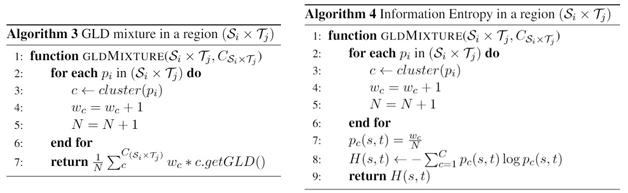
\includegraphics{figs/Algorithms_3_4.png}
\end{figure}

\subsection{Information entropy as a measure of uncertainty in a spatio-temporal region}
\label{sub:InfomationEntropyRegionWorkflow}
Now, what happens if we want to measure the uncertainty quantitatively? The information entropy is useful in this context. We use the different clusters we got in Section \ref{Clusterizing the GLD based in its lambda values} as the different outcomes of the system. The information entropy is computed as follows $H(s,t)=-\sum_{c=1}^C p_{c}(s,t)\log p_{c}(s,t)$, where $c$ represent a particular cluster in the set of clusters $C$, and $p_{c}(s,t)$ represents the probability of occurrence of the cluster $c$ in the spatio-temporal region $(s,t)$.

Algorithm 4 computes the information entropy in a region $C_{(\mathcal{S}_{i} \times \mathcal{T}_{j})}$. In lines 2 to 7, we assess the probability of each cluster in the region. Using this result, we can evaluate the information entropy $H(s, t)$, line 8, and finally, return the result in line 9.


\begin{figure}[!ht]
%\vspace{-1cm}
    \centering
    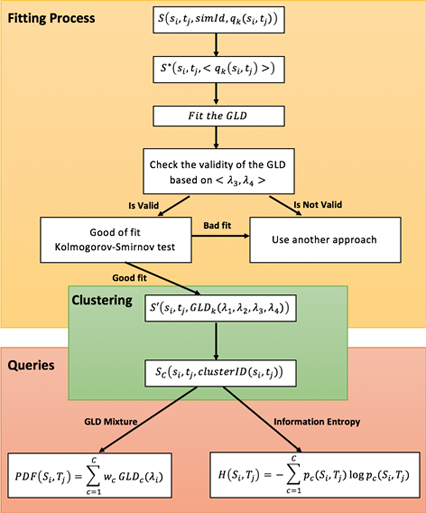
\includegraphics{figs/Diagram.png}
    \caption{SUQ$^2$ workflow divided into three steps, (a) fitting process, (b) clustering of the GLDs and, (c) queries over the results of the clustering process.}
    \label{fig:workflow}
\end{figure}

\section{Experimental Evaluation}
\label{Experiments}
In this section, we first introduce the data used in our experiments. Next, we discuss how we apply the fitting and clustering techniques over the experiment dataset. Then, we present the queries used in the performance evaluation and discuss the results expressed as a mixture of GLDs and values computed using information entropy.

As a case study, we use the HPC4e seismic benchmark, a collection of four 3D models and sixteen associated tests  \footnote{The benchmark can be freely downloaded from https://hpc4e.eu/downloads/} to generate the data of a cube. The models include simple cases that can be used in the development stage of any geophysical imaging practitioner as well as extremely large cases that can only be solved in a reasonable time using supercomputers. The models are generated based on the required size by means of a Matlab/Octave script. The tests can be used to benchmark and compare the capabilities of different and innovative seismic modelling approaches, thus simplifying the task of assessing the algorithmic and computational advantages.



\subsection{Dataset}
In the HPC4e benchmark, the models are designed as sets of 16 layers with constant physical properties. The top layer delineates the topography and the other 15 delineate different layer interface surfaces or horizons. To generate a single cube with dimensions $250\times501\times501$ we can use the values provided in the benchmark. For example, to generate a cube in the $v_{p}(m/s)$ variable we can use the fixed values of Table \ref{tab:valuesOfVp}. The first slice of this cube is shown in Figure \ref{fig:slice1}.

\begin{table}[ht]
\parbox{.45\linewidth}{
\begin{center}
    \begin{tabular}{|l|l|l|l|l|}
    \hline
    \textbf{Layer} & $v_{p}(m/s)$ &   \textbf{Layer} & $v_{p}(m/s)$ \\ \hline
    1     & 1618.92 &  9 & 2712.06\\ \hline
    2     & 1684.08 &  10 & 2532.2\\ \hline
    3     & 1994.35 &  11 & 2841.03\\ \hline
    4     & 2209.71 &   12 & 3169.31\\ \hline
    5     & 2305.55 &   13 & 3169.31\\ \hline
    6     & 2360.95 &  14 & 3642.28\\ \hline
    7     & 2381.95 &   15 & 3659.22\\ \hline
    8     & 2223.41 &   16 & 4000.00\\ \hline
    \end{tabular}
    \caption {Values of $v_{p}$ used in the generation of a single velocity field cube.}
    \label{tab:valuesOfVp}
    \end{center}
%\quad
}
%\end{table}
\parbox{.45\linewidth}{
%\begin{table}[ht]
\begin{center}
\resizebox{0.6\columnwidth}{!}{
    \begin{tabular}{|l|l|l|l|l|l|}
    \hline
    \textbf{Layer} & \textbf{PDF Family} & \textbf{Parameters} & \textbf{Layer} & \textbf{PDF Family}& \textbf{Parameters} \\\hline
    1     & Gaussian & [1619, 711.2] & 9     & Exponential & [3949, 394.9]             \\ \hline 
    2     & Gaussian & [3368, 711.2] & 10   & Exponential & [5983, 711.2]               \\ \hline
    3     & Gaussian & [8839, 711.2] & 11   & Exponential & [3520, 352.0]              \\ \hline
    4     & Gaussian & [7698, 301.5] & 12   & Exponential & [3155, 315.5]              \\ \hline
    5     & Lognormal   & [7723, 294.7] &  13   & Uniform     & [2541, 396.4]              \\ \hline
    6     & Lognormal   & [7733, 292.2] & 14   & Uniform     & [2931, 435.3]              \\ \hline
    7     & Lognormal   & [7658, 312.1] & 15   & Uniform     & [2948, 437.0]             \\ \hline
    8     & Lognormal   & [3687, 368.7] & 16   & Uniform     & [3289, 471.1]              \\ \hline
   \end{tabular}
}
    \caption {PDFs and the parameters used to sample the $v_{p}$ attribute, to generate n velocity models.}
    \label{tab:PDFsOfVp}
    \end{center}
}
\end{table}

As our purpose is to study the uncertainty in the simulation output, we need the input $v_{p}(m/s)$ to present a stochastic behavior. We model the input according to the distributions depicted in Table \ref{tab:PDFsOfVp}. Next, using a Monte Carlo method, we generate a sampling of 1000 realizations of the $v_{p}(m/s)$ variable and use a Matlab script provided by the HPC4e benchmark to generate the cube data. We perform the simulations
1000 times, one for each  realization, and generate 1000 cubes (230 GB) as output. The generated cubes are $250\times501\times501$  multi-dimensional arrays. In order to simplify the computational process and visualize the results, we select the slice 200
to be used in our experiments.
Then, we have 1000 realizations of a slice with size of $250\times501$. The data schema in Equation \ref{eq:data_base_structure} can be simplified as we only have two spatial dimensions and no time domain. Thus, the dataset can be represented as $S(x_{i},y_{j},simId,v_{p}(x_{i},y_{j}))$. In this new representation, $(x_{i},y_{j})$ is the 2D coordinates and $v_{p}(x_{i},y_{j})$ is the velocity value at point $(x_{i},y_{j})$. \textit{simId} represents the Id of the simulation, ranging from 1 to 1000.


\subsection{Fitting the GLD}\label{ft_gld}
The first step is to find the \textit{GLD} that best fits the dataset at each spatial location. Running Algorithm \ref{alg:fitGLD}, we get a new 2D array:
\begin{equation}\label{eq:gld_fit_2D}
S'(x_{i},y_{j},GLD(\lambda_{1}, \lambda_{2}, \lambda_{3}, \lambda_{4}))
\end{equation}
The raw data is significantly reduced and the new dataset is characterized by four lambda values at each spatial location. 

To check how good is the fit, we use the \textit{ks.test} algorithm included in the R-package \textit{stats} \cite{Lopes2011}, which return the \textit{p-value} at each spatial location. Our results show that the fit of the GLD is acceptable in most cases (\textit{p-value} $>0.05$),
%to be more exact, 
in 82 \% of the spatial locations (see Figure \ref{fig:p_values_greater_05}). In the 18\% regions where the GLD modeling was not acceptable, some \textit{GLD} extensions proposed in \cite{Karian2011} could be used. Since the main purpose of this paper is to demonstrate the usefulness of the \textit{GLD} in \textit{UQ}, this particular problem is beyond our scope.

\begin{figure*}[!ht]
\begin{multicols}{2}
    \centering
    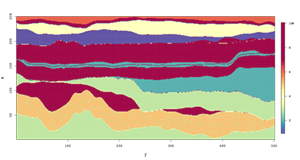
\includegraphics{figs/clusters_slice.png}
    \caption{One slice of the $250\times501\times501$ cube. In the slice, we can distinguish between the different layers.}
    \label{fig:slice1}
    \centering
    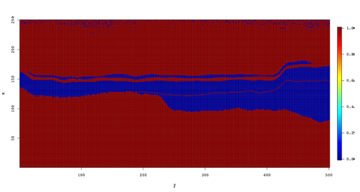
\includegraphics{figs/p_value_greater_05.png}
    \caption{The red color shows where the p-value is greater than 0.05.}
    \label{fig:p_values_greater_05}
\end{multicols}
\end{figure*}

\subsection{Clustering}\label{useCaseClustering}
Up to now, the dataset is characterized by the schema depicted by Equation \ref{eq:gld_fit_2D}. Then, using a clustering algorithm, such as k-means, we group the GLDs based on its $(\lambda_{2}, \lambda_{3}, \lambda_{4})$ values, as discussed in Section \ref{Clusterizing the GLD based in its lambda values}.
In this paper, we use the k-means algorithm with $k=10$. The choice of the clustering algorithm and the parameterization is subject for further investigation and is beyond the scope of this paper.

Once the clustering algorithm is applied, a new dataset is produced. In the new dataset,  for each spatial location, a label indicates the cluster the \textit{GLD} belongs to, as shown (see the schema at Equation \ref{eq:clustersresult}) in Figure \ref{fig:clusters}. Note that in Figure \ref{fig:clusters}, the blue region corresponding to cluster 11 is not a cluster itself. It is rather the region where the \textit{GLD} is not valid (see Section \ref{ft_gld}).

\begin{equation}\label{eq:clustersresult}
S_{\mathcal{C}}(x_{i},y_{j},clusterID, GLD_{x_{i},y_{j}})
\end{equation}

\begin{figure*}[!ht]
%\vspace{-2cm}
\begin{multicols}{2}
    \centering
        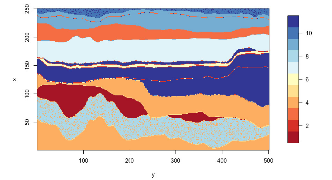
\includegraphics{figs/clusters_image.png}
    \caption{Result of the clustering using k-means with
    $k=10$.}
    \label{fig:clusters}
    \centering
    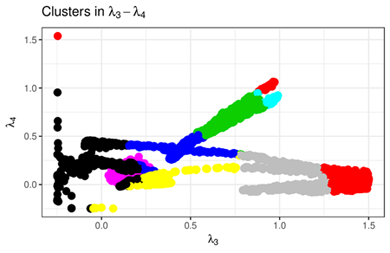
\includegraphics{figs/clusters_l3_l4.png}
    \caption{Distribution of the clusters in the $(\lambda_{3}, \lambda_{4})$ space. The points that belongs to a same cluster are one near the others, as was expected.}
    \label{fig:clusters_lambda3_lambda4_space}
\end{multicols}
\end{figure*}


If we visually compare Figure \ref{fig:slice1} with Figure \ref{fig:clusters}, we observe a close similarity. 

Another interesting result is shown in Figure \ref{fig:clusters_lambda3_lambda4_space}, where we plot the clusters in $(\lambda_{3}, \lambda_{4})$ space. As we mentioned in Section \ref{gldShape}, the shape of the \textit{GLD} depends on the values of $\lambda_{3}$ and $\lambda_{4}$. In this scenario, the expected result is that the members of the same cluster share similar values of $\lambda_{3}$ and $\lambda_{4}$. This is exactly the result we can observe in Figure \ref{fig:clusters_lambda3_lambda4_space}. 

To further corroborate this fact, Figure \ref{fig:cluster1} shows the \textit{PDFs} of 60 members of the 10 clusters. Visually assessing the figures gives an idea of how similar are the shapes of the members of a same cluster and how dissimilar are the shapes of the  members of different clusters. This suggests that our approach is valid. A product of these observations is that we can pick one member of each cluster (the centroid) as a representative of all the members of this cluster, Table \ref{tab:center_of_the_clusters}. The selected member is going to be used to answer the queries in the next Sections.
\begin{table}[ht]
\begin{center}
    \begin{tabular}{|l|l|l|l|l|l|l||l|}
    \hline
    \textbf{Cluster} & $\lambda_{2}$ & $\lambda_{3}$ & $\lambda_{4}$ & \textbf{Cluster} & $\lambda_{2}$ & $\lambda_{3}$ & $\lambda_{4}$  \\ \hline
    1     & 0.0013937313 & 0.9585829 & 1.04696461   &   6 & 0.0003894541 & 1.4076354 & -0.01925743 \\ \hline
    2     & 0.0005291388 & 1.1633978 & -0.07162550  &  7 & 0.0021972784 & 0.3253562 & 0.01493809 \\ \hline
    3     & 0.0020630696 & 0.1349486 & 0.17305941   &  8 & 0.0015421749 & 0.9491101 & 0.86699555 \\ \hline
    4     &  0.0016238358 & 0.8653824 & 0.83857646  &  9  & 0.0018672401 & 0.2176002 & 0.17862024  \\ \hline
    5     & 0.0027346929 & 0.5084664 & 0.39199164  &  10   & 0.4856397733 & 0.1404140 & 0.14011298  \\ \hline
    \end{tabular}
 \caption {Clusters centroids.}
 \label{tab:center_of_the_clusters}
 \end{center}
\end{table}

%\vspace{-5cm}
\begin{figure}[!ht]
%\vspace{-2cm}
    \centering
    %\includegraphics[scale=0.3]{figs/clusters2_s.png}
    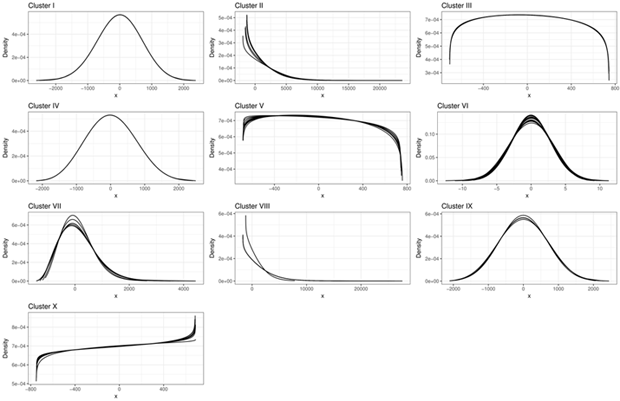
\includegraphics{figs/clusters2.png}
    \caption{\textit{PDFs} of 60 members of the 10 clusters obtained using k-means over the $(\lambda_{2}, \lambda_{3}, \lambda_{4})$ values.}
    \label{fig:cluster1}
%\end{figure}
%\vspace{0.5cm}

%\begin{figure*}
\begin{multicols}{2}
    \centering
    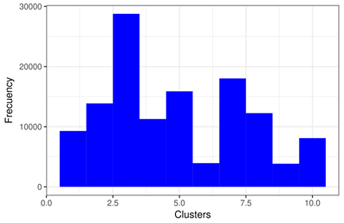
\includegraphics[scale=0.5]{figs/Clusters_histogram.png}
    %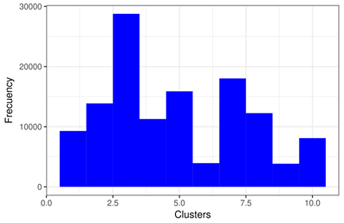
\includegraphics[bb 0 0 794 515]{figs/Clusters_histogram.png}
    \caption{Distribution of the 125250 points by clusters.}
    %\label{fig:clusters}
    \centering
    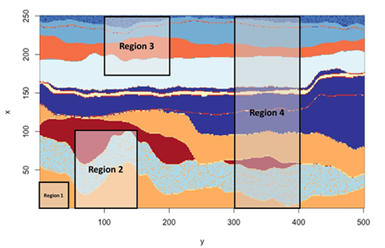
\includegraphics{figs/regions_queries.png}
    \caption{Analysis Regions. The four regions where selected intentionally in this way to warranty different distributions of the clusters inside it.}
\end{multicols}
\end{figure}

The 125250 points of the slice are distributed through the clusters following the histogram of Figure 7.

\subsection{Spatio-temporal queries}
Up to this point, the initial dataset is summarized as depicted by the schema in Equation \ref{eq:clustersresult}. It can be used to answer queries and validate our approach, by comparing the results with the raw data.

First of all, we select four spatio-temporal regions of the dataset where the clusters suggest us different behaviors. The regions are shown in Figure 8. 
With these four regions, we assess the adoption of the \textit{GLD} mixture to obtain the \textit{PDF} that characterizes the uncertainty in a specific  region (see Sections \ref{GLDmixtureresults} and \ref{informationEntropyresults}). We use the information entropy to assign a value that measures the uncertainty at each region. In Section \ref{GLDmixtureresults}, we expect the GLD mixture to characterize well the raw data, and in Section \ref{informationEntropyresults}, we hope that the information entropy is zero in region 1 and increases between regions 2, 3 and 4.

\subsubsection{GLD mixture}\label{GLDmixtureresults}
In this experiment, we use the representative \textit{GLDs} at each cluster and the weight associated to it in the region. Using these parameters, we can build a \textit{GLD mixture} that characterizes the uncertainty on that region. We use
Algorithm 3 described in Section \ref{GLDMixture}. First, we query the region to find  the clusters represented inside it, and how they are distributed. The retrieved results are shown in Table \ref{tab:distribution_of_the_clusters_by_regions}. If we divide the columns of Table \ref{tab:distribution_of_the_clusters_by_regions} by the sum of the elements of each column, we get the weight needed to formulate the \textit{mixed GLDs}. It is clear that the \textit{GLD} in region 1 is represented by the \textit{GLD} of cluster 4. In the other three cases, we get what is shown in the set of 
equations \ref{eq:gld_mix}.


\begin{table}[!ht]
%\vspace{-0.5cm}
\begin{center}
\scalebox{0.6}{
    \begin{tabular}{|l|l|l|l|l|}
    \hline
    \textbf{Cluster} & \textbf{Region 1} &  \textbf{Region 2} &  \textbf{Region 3} &   \textbf{Region 4}  \\ \hline
    1     & 0   		& 2250 & 0 & 979            \\ \hline
    2     & 0   		& 0 & 0 & 268           \\ \hline
    3     & 0      	& 0 & 2596 & 1468       \\ \hline
    4     & 1640	& 4467 & 0 & 5173         \\ \hline
    5     & 0       & 149 & 0 & 269          \\ \hline
    6     & 0     & 0 & 0 & 416           \\ \hline
    7     & 0       & 0 & 1967 & 3920           \\ \hline
    8     & 0     & 3335 & 0 & 3432             \\ \hline
    9     & 0      & 0 & 1918 & 3280       \\ \hline
    10   & 0      & 0 & 901 & 583         \\ \hline
    \end{tabular}}
    \caption {Distribution of the clusters by regions. The four regions are selected intentionally this way to warrant different distributions of the clusters inside it.}
    \label{tab:distribution_of_the_clusters_by_regions}
    \end{center}
\end{table}


\begin{align}
%\vspace{-0.2cm}
\begin{split}
\label{eq:gld_mix}
GLD_{region2} = 0.22GLD_{c1} + 0.44GLD_{c4} + 0.014GLD_{c5} + 0.33GLD_{c8} \\
 GLD_{region3} = 0.34GLD_{c3} + 0.26GLD_{c7} + 0.25GLD_{c9} + 0.12GLD_{c10} \\
 GLD_{region4} = 0.22GLD_{c1} + 0.44GLD_{c4} + 0.014GLD_{c5}  + 0.33GLD_{c8}
\end{split}
\end{align}


Now, we need to evaluate whether the \textit{mixture of GLDs} correctly models the uncertainty in a region. We perform the same \textit{ks-test} used to evaluate the
good quality of the fit, described in Section \ref{gldFitProcess}. Based on the \textit{p-value}, Table \ref{tab:p_values_by_regions}, we can conclude that in all 4 regions the \textit{mixture of GLDs} is a good fit to the raw data.

\begin{table}[ht]
\begin{center}
    \begin{tabular}{|l|l|l|l|l|}
    \hline
    \textbf{Metrics} & \textbf{Region 1} &  \textbf{Region 2} &  \textbf{Region 3} &   \textbf{Region 4}  \\ \hline
    p-value     & 0.73   		& 0.56 & 0.34 & 0.08            \\ \hline
    \end{tabular}
    \caption {p-values by regions.}
    \label{tab:p_values_by_regions}
    \end{center}
\end{table}



\subsubsection{Information Entropy}\label{informationEntropyresults}

Based on the distribution of clusters inside the regions (see Table \ref{tab:distribution_of_the_clusters_by_regions}), we can compute the entropy. 

\begin{table}[ht]
\begin{center}
    \begin{tabular}{|l|l|l|l|l|}
    \hline
    \textbf{entropy} & \textbf{Region 1} &  \textbf{Region 2} &  \textbf{Region 3} &   \textbf{Region 4}  \\ \hline
    value     & 0   		& 1.122243 & 1.41166 & 2.024246            \\ \hline
    \end{tabular}
    \caption {Information Entropy by regions.}
    \label{tab:entropy_by_regions}
    \end{center}
\end{table}

As we expect (see Table \ref{tab:entropy_by_regions}), the entropy in region 1 is zero, because the region contains only members of the cluster 4. On the other regions the entropy increases from region 2 to region 4, as expected. The information entropy is a very good and simple measure of the uncertainty, and here it is demonstrated its usefulness combined with the \textit{GLD}.

 

\section{Conclusion}
\label{Conclusions}

In this paper, we proposed SUQ$^2$, a method to answer uncertainty quantification (UQ) queries over large spatio-temporal simulations. SUQ$^2$ trades large simulation data by probability density functions (PDFs), thus saving huge amount of storage space and computational cost. It enables complex data distribution representation at each simulation point, as much as a  spatio-temporal view  of simulation uncertainty computed by mixing spatial point PDFs.
We evaluated SUQ$^2$ using a seismology use case, considering the computation of uncertainty in regions of a slice of the seismic cube. The results show that SUQ$^2$ method produces an accurate view of the uncertainty in regions of space-time while considerably saving storage space and reducing the cost associated with the PDF modeling of the dataset. To the best of our knowledge, this is the first work to use GLD as the basis for answering UQ queries in spatio-temporal regions and to compile a series of techniques to produce a query answering workflow.



\subsection*{Acknowledgments}
This work has been funded by CNPq, CAPES, FAPERJ, the Inria HPDaSc
and SciDISC Associated Teams and the European Commission (HPC4E H2020) project.


\itemsep=1pt
\begin{thebibliography}{10}
\begin{small}


\bibitem{Tobergte2013}
D. R. Tobergte and S. Curtis.
\newblock {Workshop on Quantification, Communication, and Interpretation of
  Uncertainty in Simulation and Data Science}.
\newblock in {\em Journal of Chemical Information and Modeling}, 53(9):1689--1699,
  2013.


\bibitem{Baroni2014a}
G. Baroni and S. Tarantola.
\newblock {A General Probabilistic Framework for uncertainty and global
  sensitivity analysis of deterministic models: A hydrological case study}.
\newblock in {\em Environmental Modelling and Software}, 51:26--34, 2014.

\bibitem{Johnstone2015}
R. H. Johnstone, E. T. Y. Chang, R. Bardenet, T. P. de~Boer,
  D. J. Gavaghan, P. Pathmanathan, R. H. Clayton, and G. R. Mirams.
\newblock {Uncertainty and variability in models of the cardiac action
  potential: Can we build trustworthy models?}
\newblock in {\em Journal of Molecular and Cellular Cardiology}, 96:49--62, 2016.
  


\bibitem{Karian2011}
Z. A. Karian and E. J. Dudewicz.
\newblock {\em {Handbook of fitting statistical distributions with R}}.
\newblock 2011.


\bibitem{Freimer1988}
M. Freimer, C. T. Lin, and G. S. Mudholkar.
\newblock {A Study Of The Generalized Tukey Lambda Family}.
\newblock in {\em Communications in Statistics - Theory and Methods},
  17(10):3547--3567, 1988.
  
\bibitem{Corlu2016}
C. G. Corlu and M. Meterelliyoz.
\newblock {Estimating the Parameters of the Generalized Lambda Distribution:
  Which Method Performs Best?}
\newblock in {\em Communications in Statistics: Simulation and Computation},
  45(7):2276--2296, 2016.
  

\bibitem{Su2007}
S. Su.
\newblock {Fitting Single and Mixture of Generalized Lambda Distributions to
  Data via Discretized and Maximum Likelihood Methods: GLDEX in R}.
\newblock {\em Journal of Statistical Software}, 21(9), 2007.

\bibitem{Lampasi2006}
D. A. Lampasi, F. Di Nicola, and L. Podesta.
\newblock {Generalized lambda distribution for the expression of measurement
  uncertainty}.
\newblock {\em IEEE Transactions on Instrumentation and Measurement},
  55(4):1281--1287, 2006.
  
\bibitem{Movahedi2013}
M. M. Movahedi, M. R. Lotfi, and M. Nayyeri.
\newblock {A solution to determining the reliability of products Using
  Generalized Lambda Distribution}.
\newblock {\em Research Journal of Recent Sciences Res.J.Recent Sci},
  2(10):41--47, 2013.
  
 \bibitem{Ning2008}
W. Ning, Y. Gao, and E. J. Dudewicz.
\newblock {Fitting mixture distributions using generalized lambda distributions
  and comparison with normal mixtures}.
\newblock {\em American Journal of Mathematical and Management Sciences},
  28(1-2):81--99, 2008.
  
\bibitem{Wellmann2012}
J. F. Wellmann and K. R. Lieb.
\newblock {Uncertainties have a meaning: Information entropy as a quality
  measure for 3-D geological models}.
\newblock {\em Tectonophysics}, 526-529:207--216, 2012.

\bibitem{Liu2019}
J. Liu,N. Lemus, E. Pacitti, F. Porto, P.  Valduriez. \newblock {Parallel computation of PDFs on big spatial data using spark}. \newblock in {em Distributed and Parallel Databases}, pp. 1-28. In press, 10.1007/s10619-019-07260-3, 2019.

\bibitem{Lopes2011}
R. H. C. Lopes  \newblock {Kolmogorov-Smirnov Test.} \newblock in {Lovric M. (eds) International Encyclopedia of Statistical Science. Springer, Berlin, Heidelberg}, 2011.

\bibitem{Ramberg1974} J. S. Ramberg, and B. W. Schmeiser.\newblock {An approximate
method for generating asymmetric random
variables}. \newblock in {em Communications of the ACM}, 17(2), 78–82.
doi:10.1145/360827.360840, 1974.


\end{small}
 \end{thebibliography}
\end{document}

\endinput
%%
%% End of file `elsarticle-template-harv.tex'.
